\begin{frame}
\frametitle{Electronic Flight Bags}
\begin{center}
Aeronautical Data and Information
\end{center}
\end{frame}

\begin{frame}
\frametitle{CASR1988 REG 175}
\begin{block}{What is CASR1998 REG 175 about?}
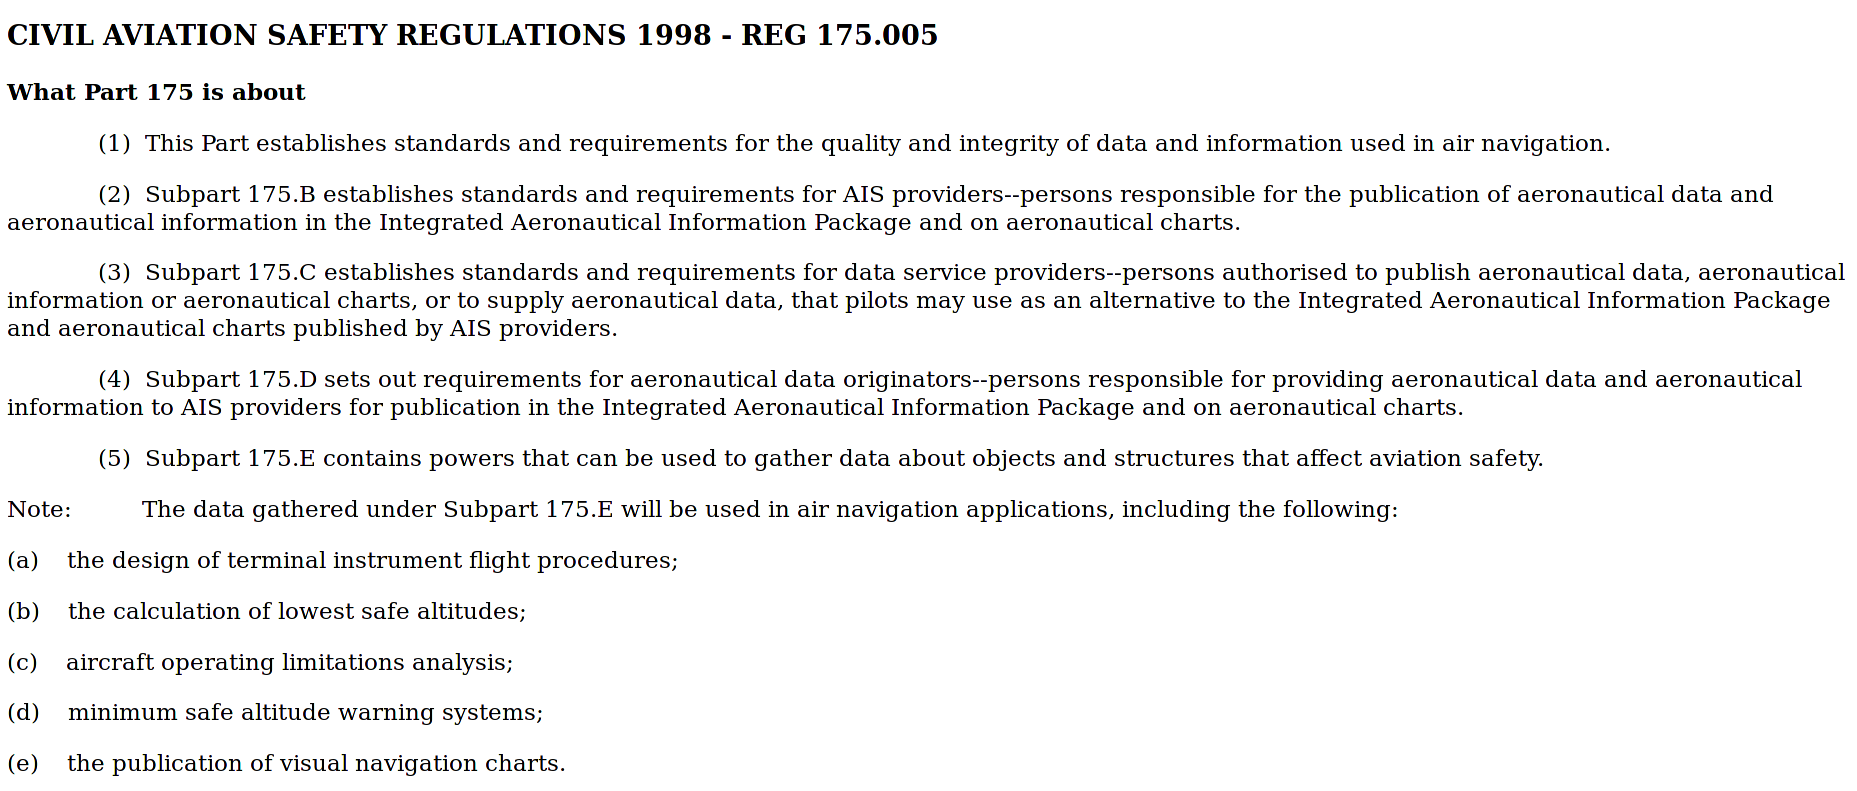
\includegraphics[height=0.5\textheight]{image/casr175_005.png}
\end{block}
\par
``(e) the publication of visual navigation charts.''
\end{frame}

\begin{frame}
\frametitle{CAR1988 REG 233(1)(h) \emph{moved to CASR1998 REG 175}}
\scriptsize
\begin{block}{CAR1988 REG 233(1)(h)}
The pilot in command of an aircraft must not commence a flight if he or she has not received evidence, and taken such action as is necessary to ensure, that:
\par
\ldots
\par
(h)  the aeronautical data and aeronautical information mentioned in subregulation (1A) is carried in the aircraft and is readily accessible to the flight crew.
\end{block}
\par
\end{frame}

\begin{frame}
\frametitle{VTC/VNC}
\begin{block}{This is a Brisbane Visual Terminal Chart (VTC)}
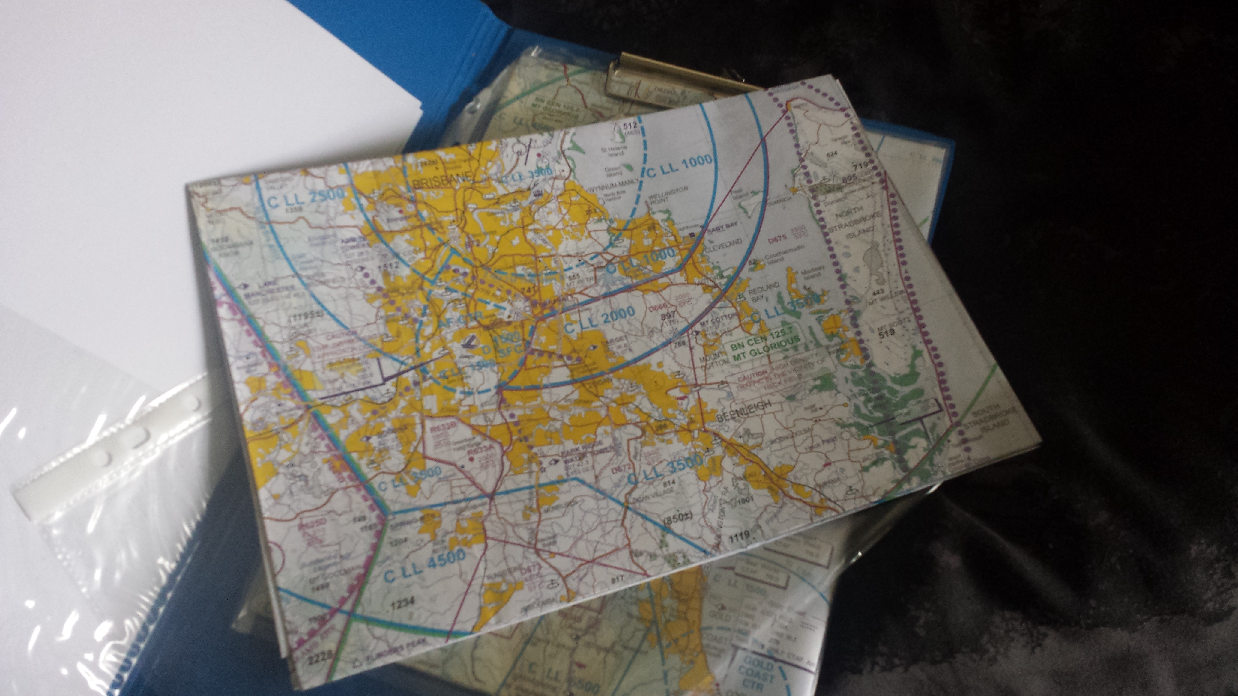
\includegraphics[height=0.3\textheight]{image/vtc.png}
\begin{itemize}
\item<1-> It unfolds out to 500mm x 1000mm.
\item<2-> Updated every 3 months (approx).
\end{itemize}
\end{block}
\end{frame}

\begin{frame}
\frametitle{VTC/VNC}
\begin{block}{Under CAR1988 REG 133(1)(h)}
\begin{itemize}
\item<1-> These charts are required on every flight.
\item<2-> Reading them during flight is physically impractical.
\item<3-> Instead, memorise the important parts.
\item<4-> If they must be read, measure against risks of diverting eyes inside.
\end{itemize}
\end{block}
\end{frame}

\begin{frame}
\frametitle{VTC/VNC}
\begin{block}{Surely these exist in electronic format?}
Why yes, they do.
\end{block}
\end{frame}

\begin{frame}
\frametitle{VTC/VNC}
\large
\begin{center}
but
\end{center}
\end{frame}

\begin{frame}
\frametitle{CASR1998 REG 175.145(1)}
\begin{block}{AIS providers--publication of aeronautical charts relating to areas etc. outside authority}
(1) This regulation applies if an AIS provider publishes an aeronautical chart that includes aeronautical data or aeronautical information that relates to an area, aerodrome, airspace or ATS route not covered by the provider's certificate.
\end{block}
\end{frame}
\begin{frame}
\frametitle{CASR1998 REG 175.145(1)}
\large
\begin{center}
No problem.
\par
Let's use approved electronic AIS aeronautical charts.
\end{center}
\end{frame}

\begin{frame}
\frametitle{CASR1998 REG 175.145(1)}
\large
\begin{center}
but
\end{center}
\end{frame}

\begin{frame}
\frametitle{CASR1998 REG 175.145(1)}
\large
\begin{center}
the paper charts are the authoritative, approved data source.
\end{center}
\end{frame}

\begin{frame}
\frametitle{CASR1998 REG 175.145(1)}
\begin{block}{let's fly across .jpg files}
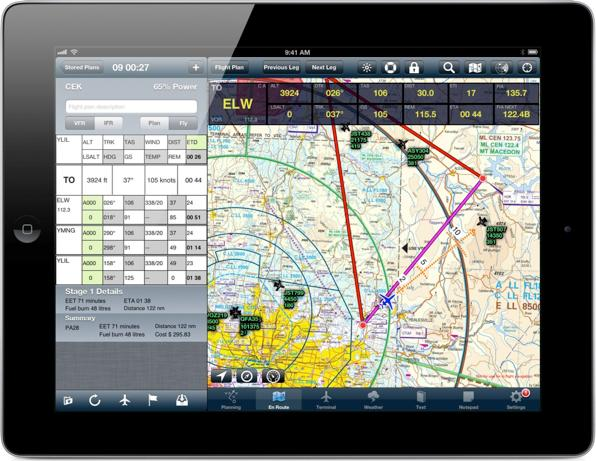
\includegraphics[height=0.5\textheight]{image/avplan-screenshot.jpg}
\end{block}
\end{frame}

\begin{frame}
\frametitle{CASR1998 REG 175.145(1)}
\begin{block}{that do not accurately georectify}

\includegraphics[height=0.5\textheight]{image/georectification.png}
\end{block}
\end{frame}

\begin{frame}
\frametitle{CASR1998 REG 175}
\begin{block}{is accuracy important?}
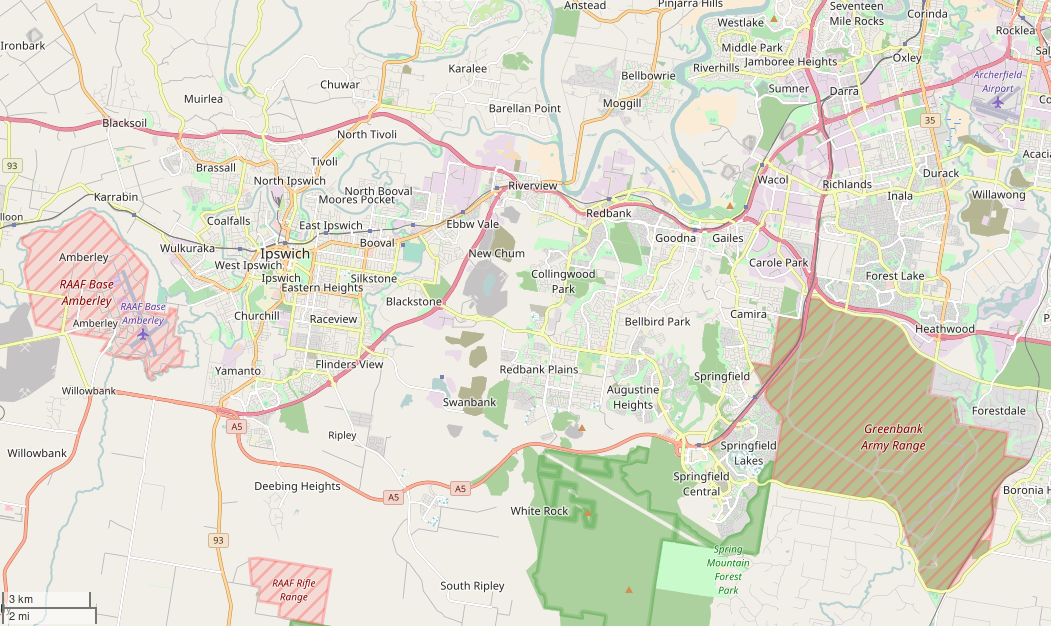
\includegraphics[height=0.5\textheight]{image/map-amberley-greenbank.png}
\end{block}
\end{frame}

\begin{frame}
\frametitle{CASR1998 REG 175}
\begin{block}{Yes}
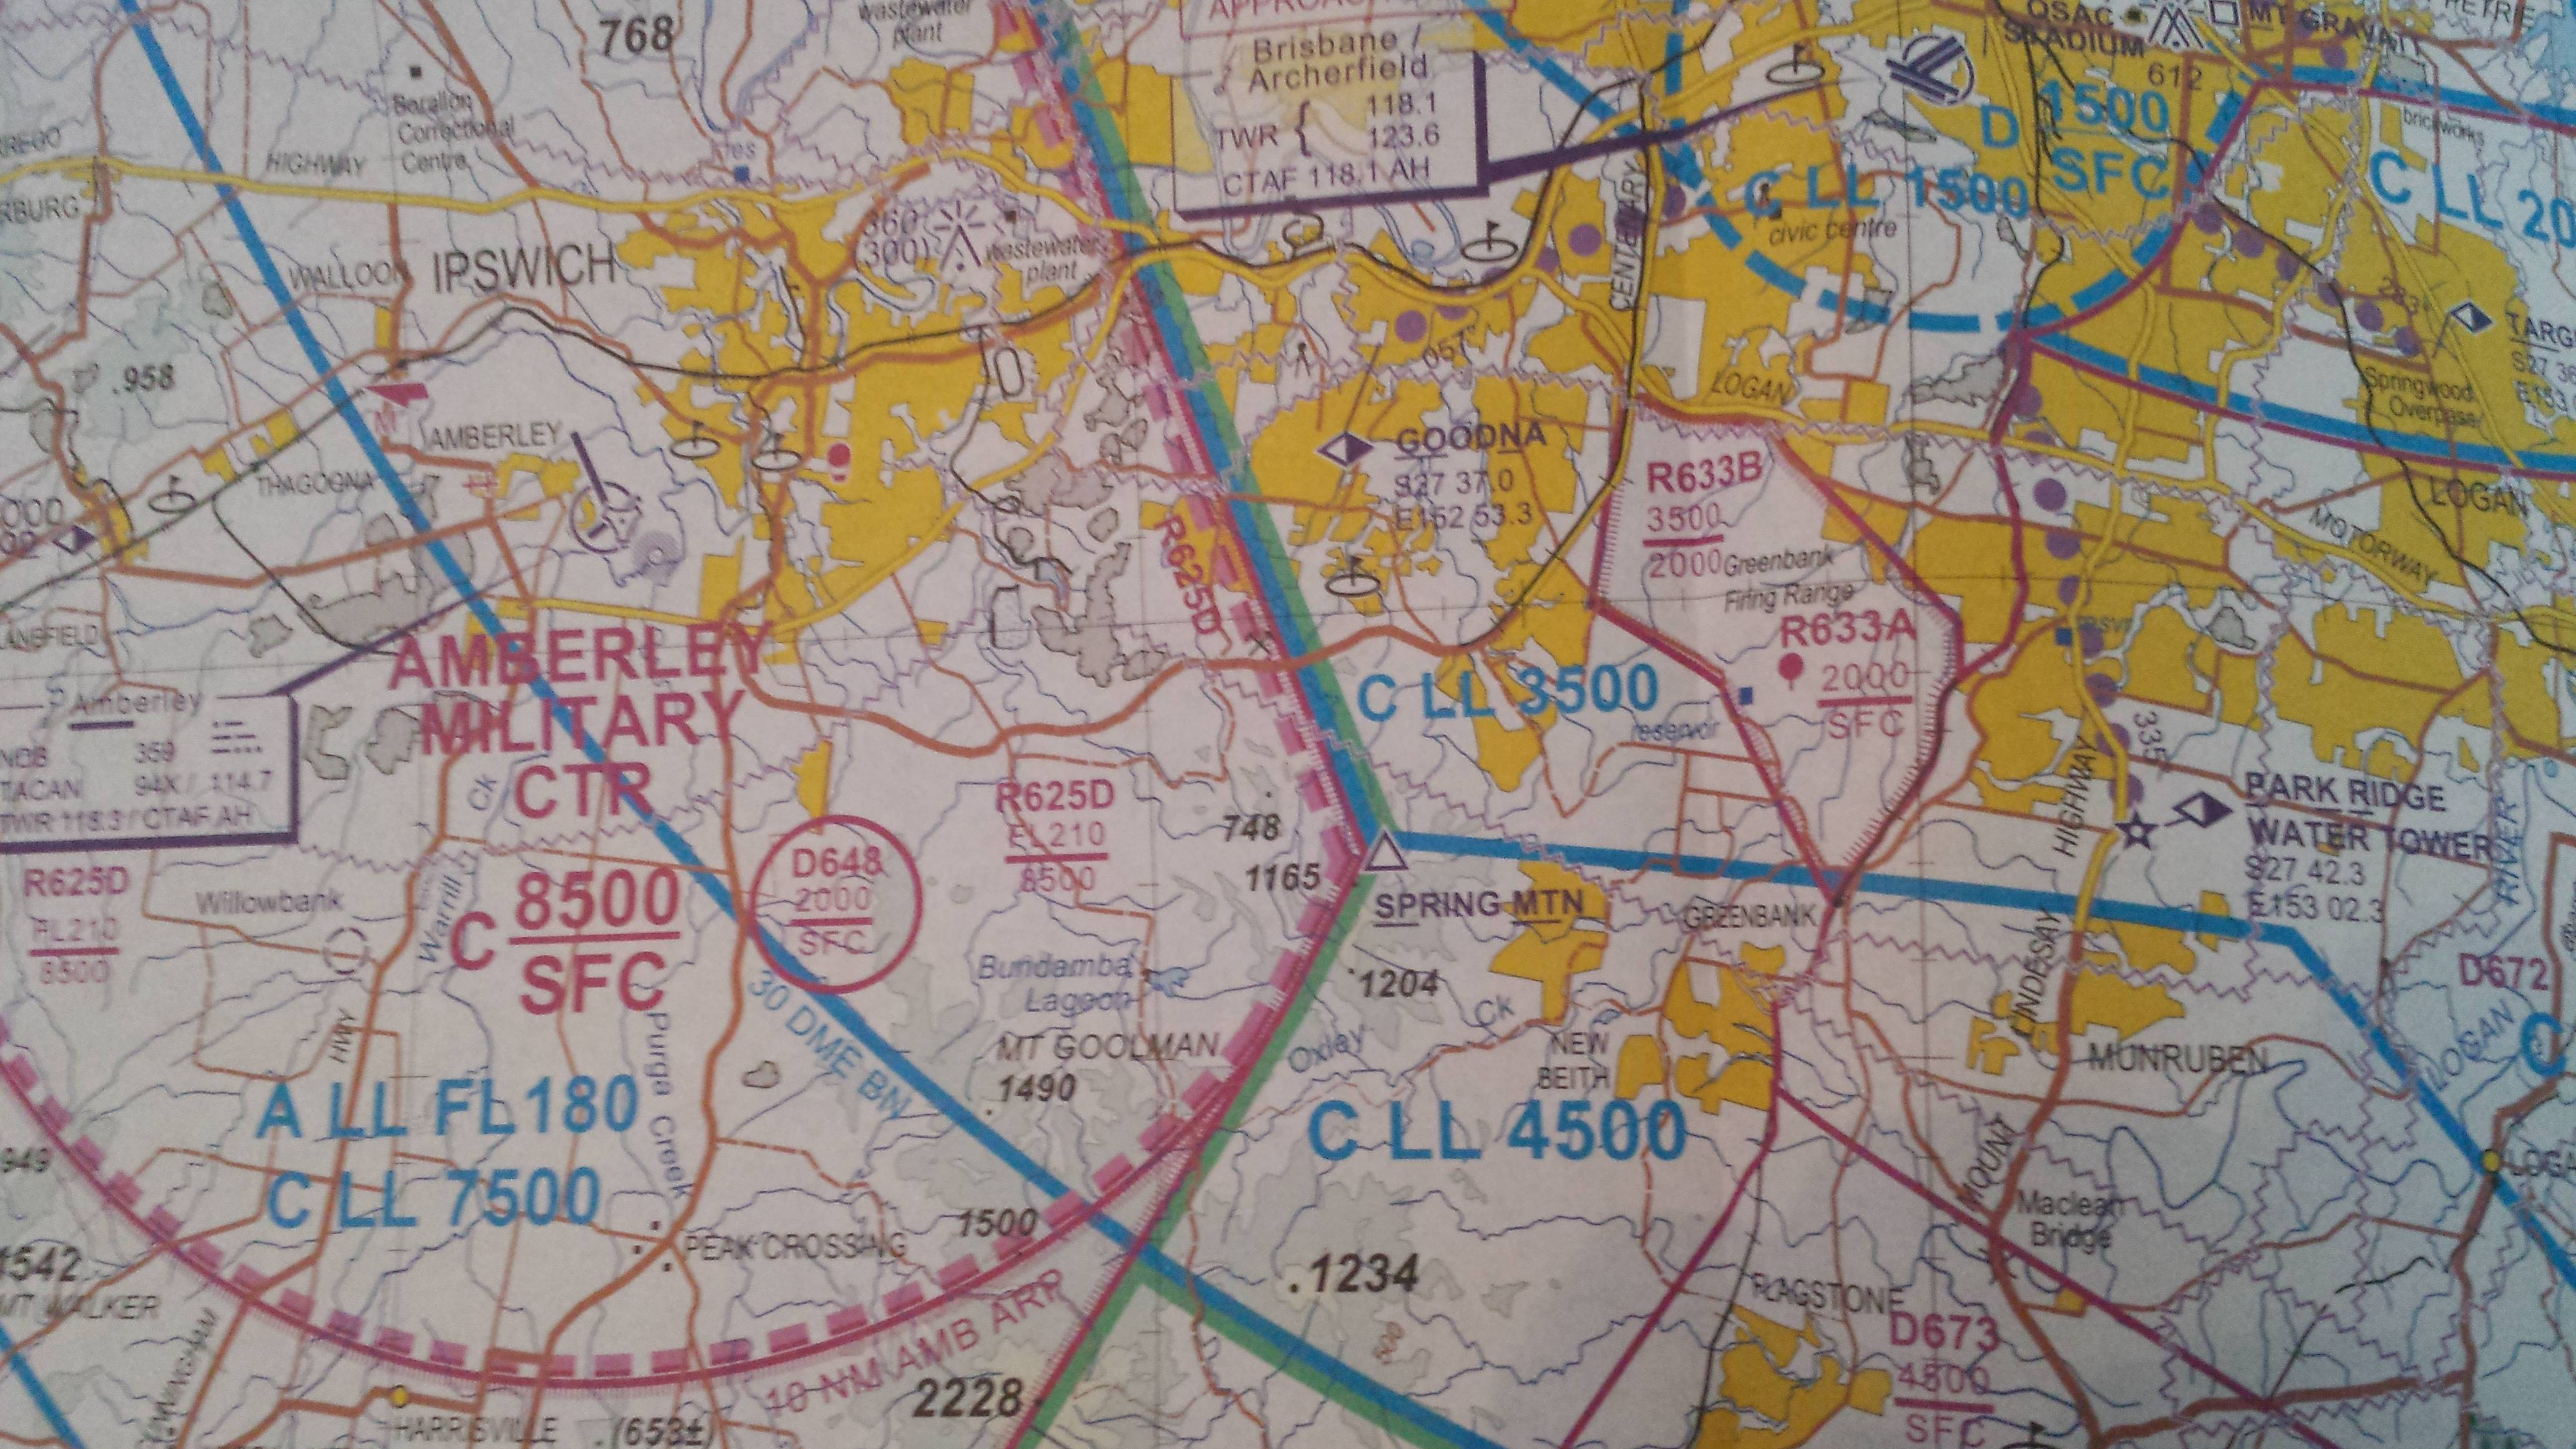
\includegraphics[height=0.5\textheight]{image/vtc-amberley-greenbank.jpg}
\begin{itemize}
\item \tiny{Amberley RAAF is conditionally \textbf{RA1}}
\item \tiny{Greenbank Army is \textbf{RA3} SFC to 2000}
\end{itemize}
\end{block}
\end{frame}

\begin{frame}
\frametitle{CASR1998 REG 175}
\begin{block}{My nightmares are made of this stuff \tiny{\emph{(AIP EMERG 5.12)}}}
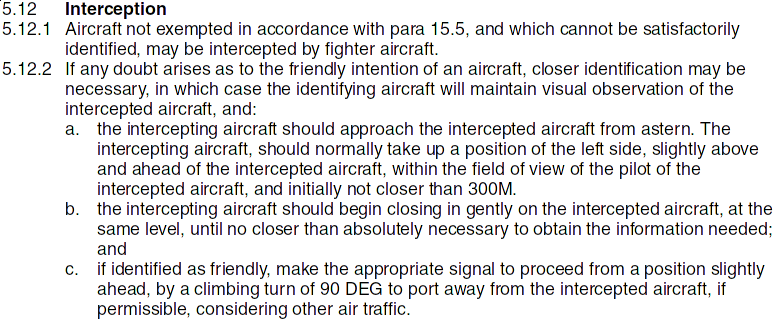
\includegraphics[height=0.5\textheight]{image/ersa-interception.png}
\end{block}
\end{frame}

\begin{frame}
\frametitle{CASR1998 REG 175}
\begin{block}{Alternatively}
\begin{center}
Use non-certificated aeronautical data with restrictions on operations.
\end{center}
\end{block}
\end{frame}

\begin{frame}
\frametitle{uncertificated aeronautical data}
\large
\begin{center}
but
\end{center}
\end{frame}

\begin{frame}
\frametitle{New Zealand CAA}
\begin{block}{Fatal Accident Report ZK-SML, Mount Duppa, 09 April 2011. \textbf{CFIT}}
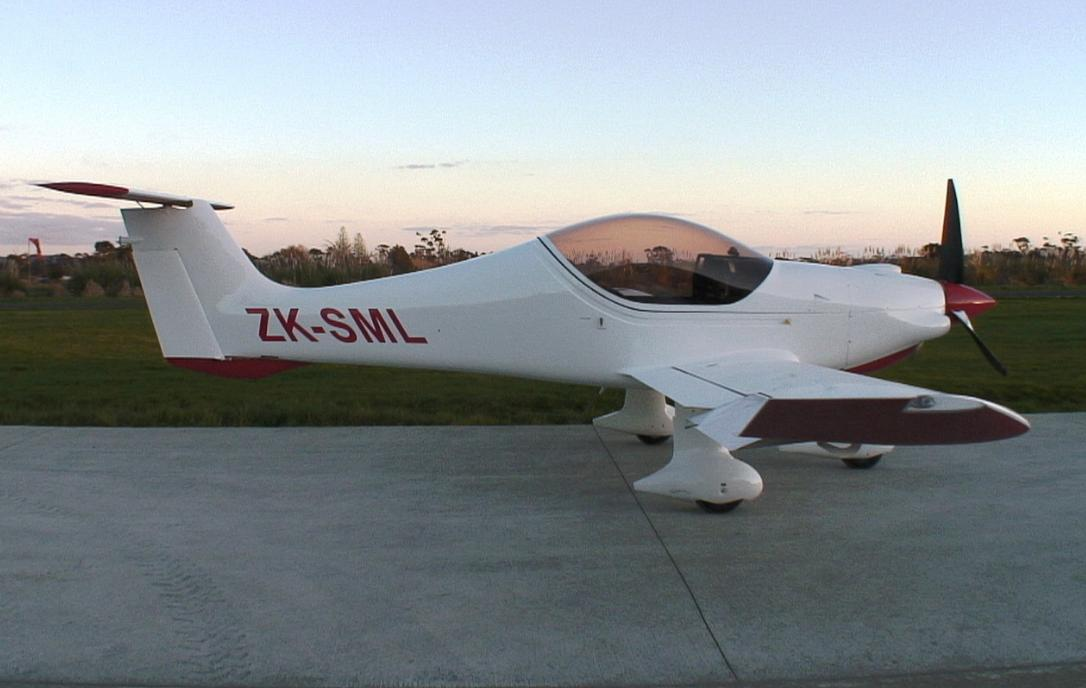
\includegraphics[height=0.5\textheight]{image/zk-sml.jpg}
\end{block}
\end{frame}

\begin{frame}
\frametitle{ZK-SML}
\begin{block}{VFR into IMC}
\begin{itemize}
\item<1-> VFR into IMC is a dangerous flight condition where a visual pilot is required to maintain, but has lost, outside visual reference e.g. due to flying into cloud
\item<2-> It is particularly dangerous if the pilot is untrained and/or the aircraft is ill-equipped to handle instrument (non-VFR) conditions
\item<3-> ZK-SML is a light, VFR only, experimental aircraft with \textbf{lots} of modern technology onboard
\end{itemize}
\end{block}
\end{frame}

\begin{frame}
\frametitle{ZK-SML}
\begin{block}{Accident Report excerpt \tiny{\emph{(1.16.1)}}}
\begin{quote}
Assistance was sought from the New Zealand agent for the MGL Avionics EFIS system installed in the aircraft.  While reviewing the aircraft's flight path based on the SSR data on a computer based simulator, two major errors in the EFIS navigation software were discovered. 
\end{quote}
\end{block}
\end{frame}

\begin{frame}
\frametitle{ZK-SML}
\begin{block}{Accident Report excerpt \tiny{\emph{(Figure 2)}}}
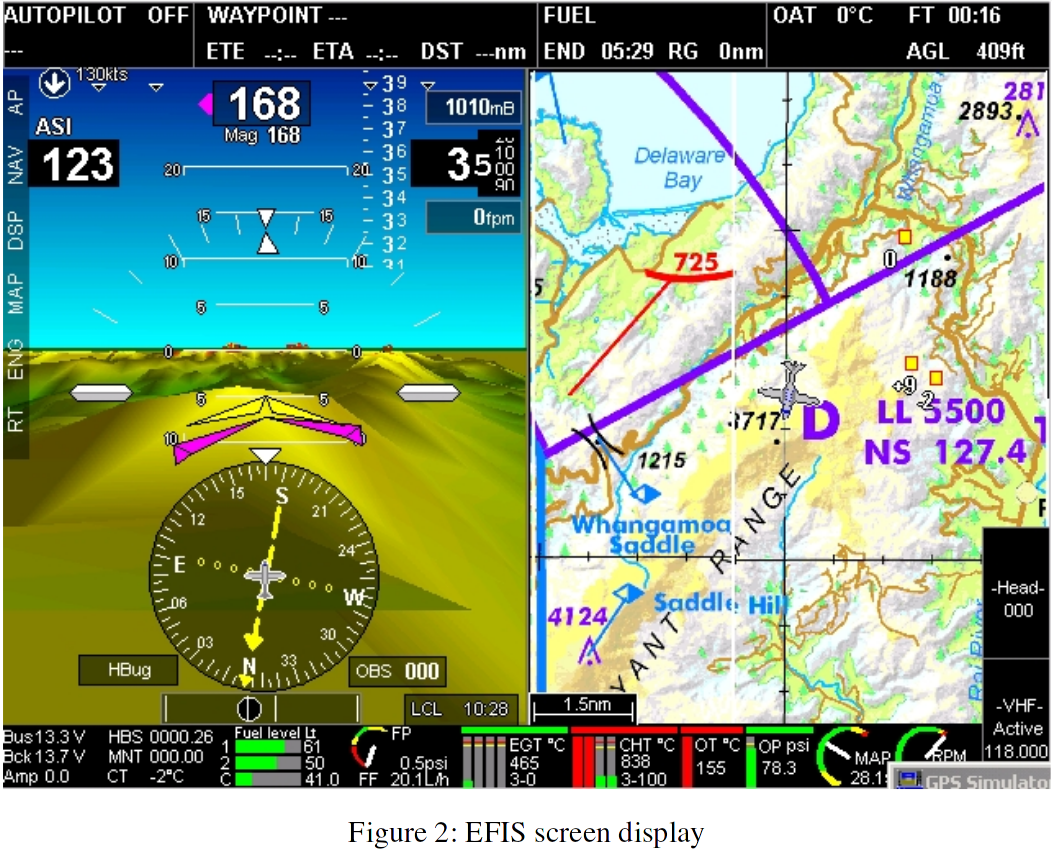
\includegraphics[height=0.7\textheight]{image/zk-sml-map.png}
\end{block}
\tiny{At what height is the terrain at this aeroplane's 12 o'clock position?}
\end{frame}

\begin{frame}
\frametitle{ZK-SML}
\begin{block}{Accident Report excerpt \tiny{\emph{(1.16.2)}}}
\begin{quote}
It was found that the moving map display did not accurately display the 3717 feet spot height for Mount Duppa.  Due to the positioning of a map join which passes through the `3', the spot height for Mount Duppa was corrupted and was displayed as 1717 feet.  Refer to the spot height next to the aircraft symbol on the map display in figure 2. 
\end{quote}
\end{block}
\end{frame}

\begin{frame}
\frametitle{Aeronautical charts}
\begin{block}{}
This is a real VTC, marked for a planned visual navigation exercise
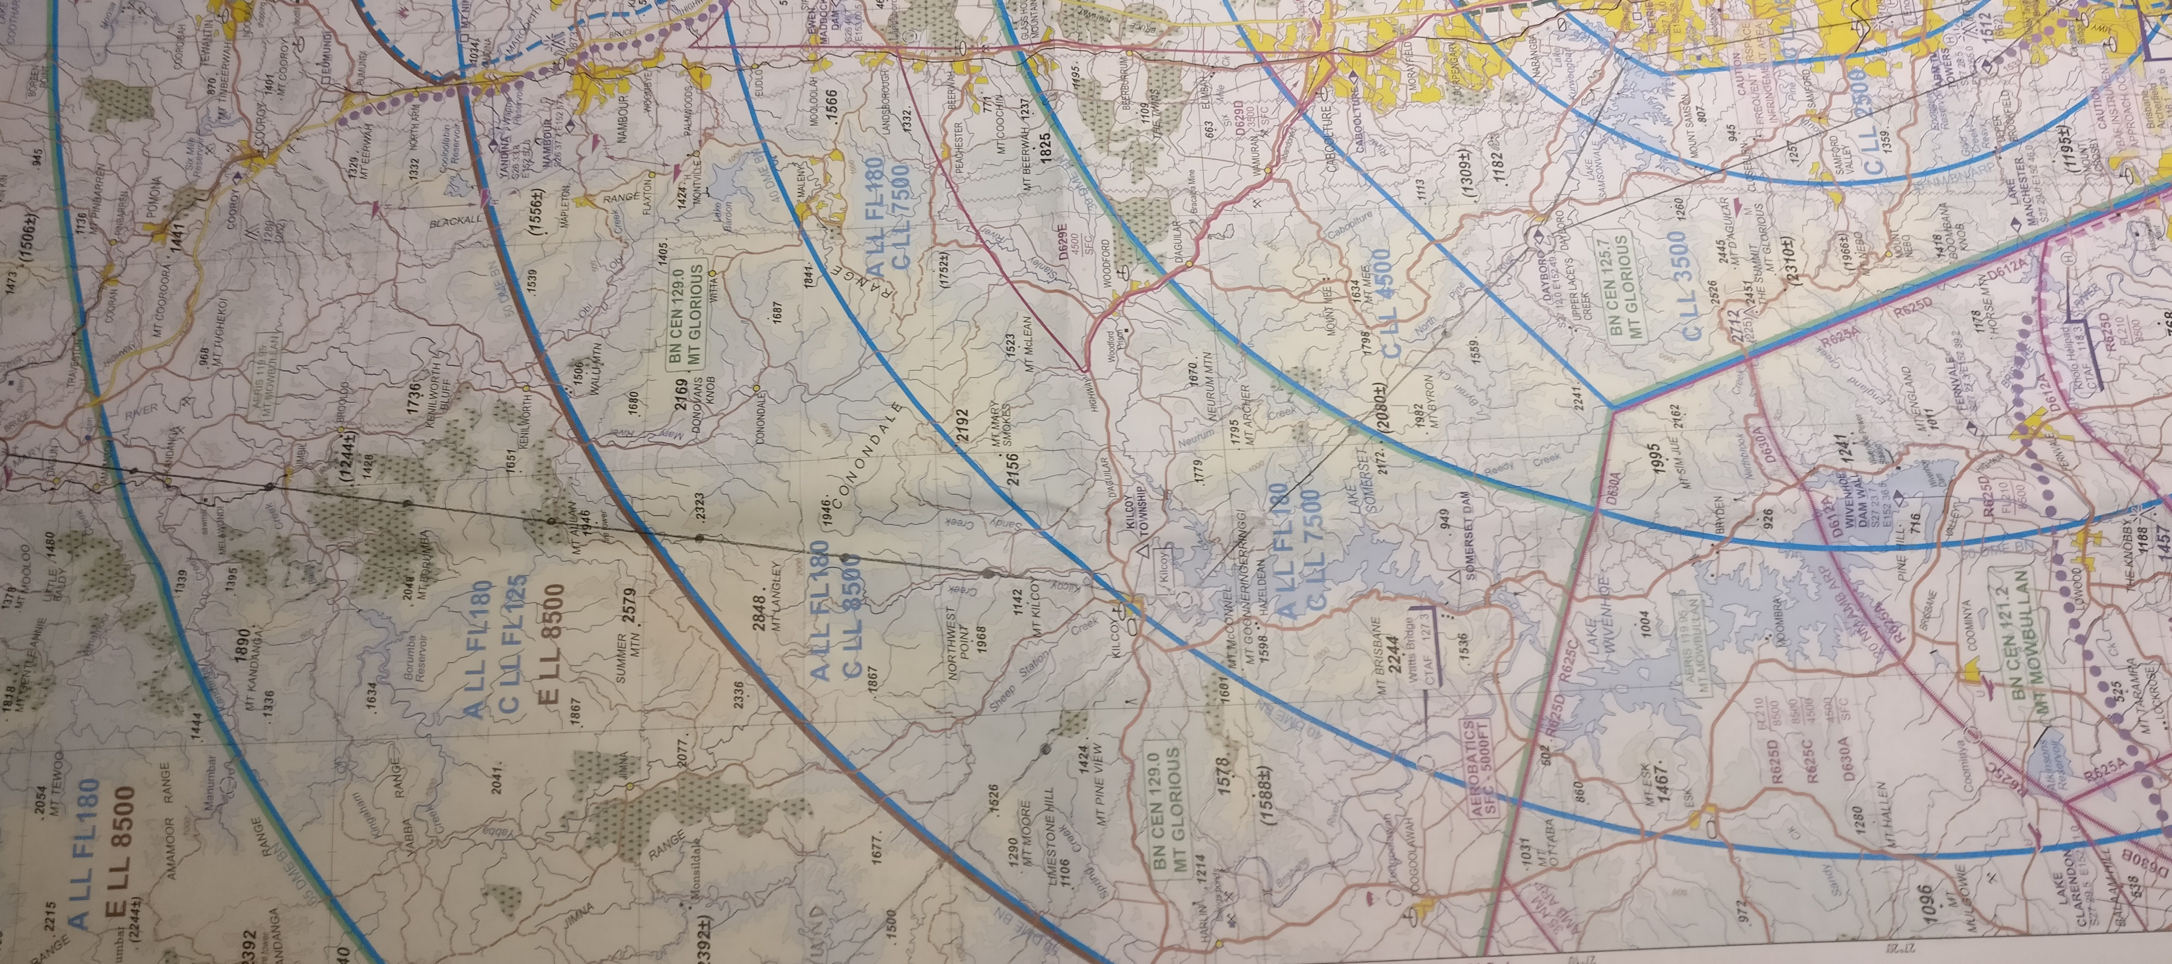
\includegraphics[height=0.5\textheight]{image/planned-vtc00-resize50.png}
\begin{itemize}
\item \tiny{scale 1:250000}
\item \tiny{folded, according to planned route}
\item \tiny{pencil marked according to planned route}
\item \tiny{pencil marks at 10nm intervals for DR exercise}
\item \tiny{note Brisbane airspace boundaries in blue}
\item \tiny{note radio frequencies and boundaries in green}
\end{itemize}
\end{block}
\end{frame}

\begin{frame}
\frametitle{Aeronautical charts}
\begin{block}{}
This is a real WAC, marked for the same planned exercise
\includegraphics[height=0.6\textheight]{image/planned-wac00-resize50.png}
\begin{itemize}
\item \tiny{scale 1:1000000}
\item \tiny{relevant airspace boundaries are transferred (red)}
\item \tiny{relevant radio frequency boundaries are transferred (green)}
\item \tiny{diversion is an integral part of the navigation exercise \textemdash{ revert to VTC}}
\end{itemize}
\end{block}
\end{frame}

{
\usebackgroundtemplate{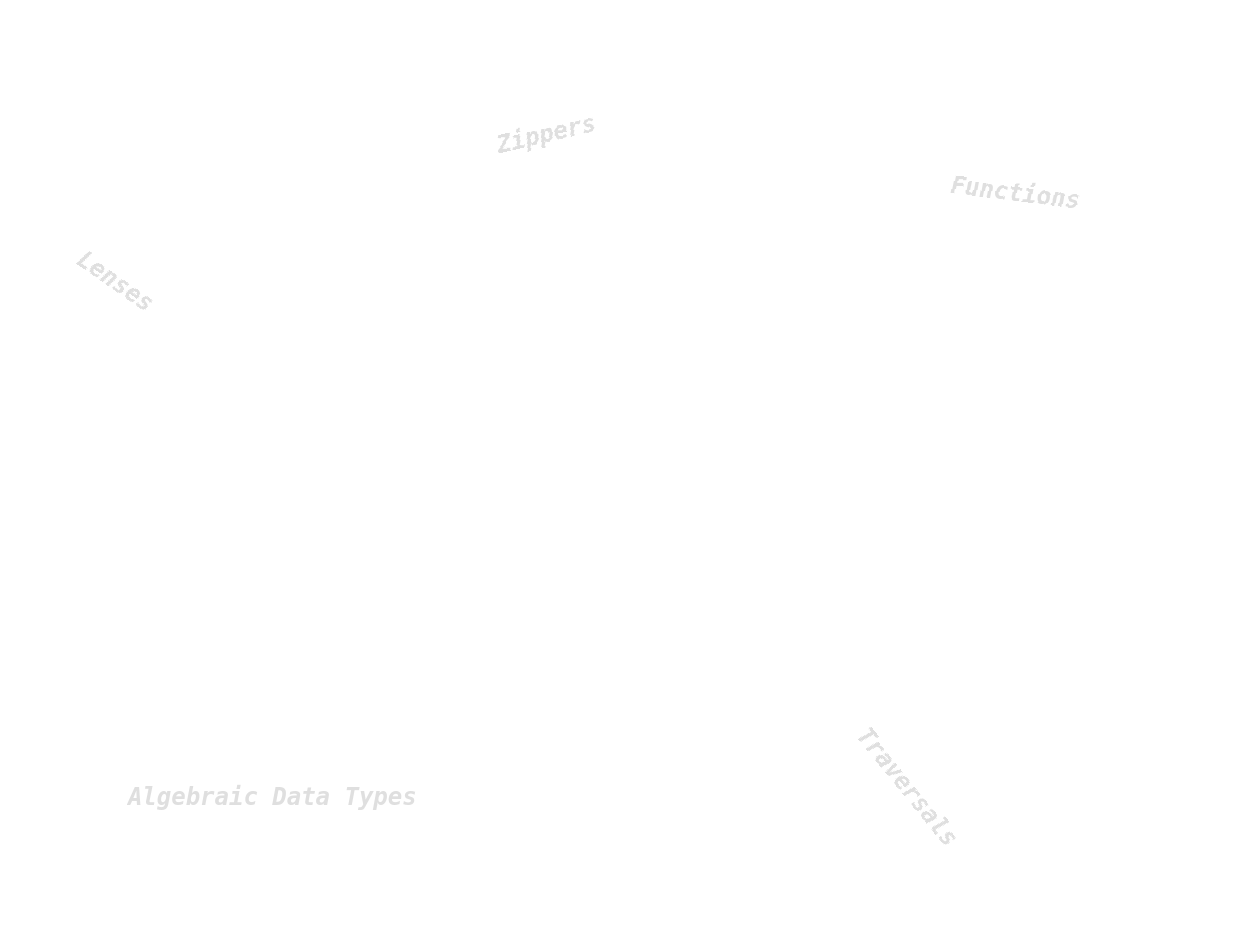
\includegraphics[width=\paperwidth]{image/data-types-background.png}} {}
\begin{frame}
\frametitle{Aeronautical charts}
\begin{center}
Don't we already have sound solutions to these problems?
\end{center}
\end{frame}
}